\documentclass[task=1]{exercise}

\setgroup{Basiskurs Physik}
\settitle[Arbeitsblatt 1]{Elektrisches Feld}
\addstudent{Schuljahr 22/23}
\addstudent{Jahrgangsstufe J2}

\renewcommand{\vec}{\overrightarrow}

\begin{document}
  \task[Coulomb-Kraft zwischen zwei Punktladungen I]
  Es befinde sich eine positive Punktladung $Q_1 = e = 1,602 \cdot 10^{-19}\,\mathrm{C}$ im Punkt $(0,0)$.

  Weiterhin befindet sich am Ort $\vec{r} = (x,y)$ eine positive Punktladung $q = e = 1,602 \cdot 10^{-19}\,\mathrm{C}$.
  
  Zeichne f\"ur alle unten eingetragenen F\"alle von $\vec{r}$ die Coulomb-Kraft im Ma{\ss}stab
  \begin{equation}
    1\,\mathrm{cm} \,\,\, \hat{=}\,\,\, \frac{k\cdot e^2}{\left( 5{,}3\cdot 10^{-11}\, \mathrm{m} \right)^2}
  \end{equation}
  ein.
  
  \vspace{2cm}
  
  \begin{center}
   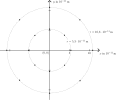
\includegraphics{images/diagram.pdf}
  \end{center}



\newpage
  
  \task[Coulomb-Kraft zwischen zwei Punktladungen II]
    Nun habe die positive Punktladung am Ort $(0,0)$ eine Ladung $Q_2 = 2e = 3,204 \cdot 10^{-19}\,\mathrm{C}$ .
  Wieder befinde sich am Ort $\vec{r} = (x,y)$ eine positive Punktladung $q = e = 1,602 \cdot 10^{-19}\,\mathrm{C}$.
  
  Zeichne f\"ur alle unten eingetragenen F\"alle von $\vec{r}$ die Coulomb-Kraft im Ma{\ss}stab
  \begin{equation}
    1\,\mathrm{cm} \,\,\, \hat{=}\,\,\, \frac{k\cdot e^2}{\left( 5{,}3\cdot 10^{-11}\, \mathrm{m} \right)^2}
  \end{equation}
  ein.
  
  \vspace{2cm}
  
  \begin{center}
   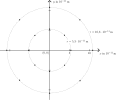
\includegraphics{images/diagram.pdf}
  \end{center}
  
  \vspace{2cm}
  
  Vergleiche mit dem Diagramm aus Aufgabe 1.
  
\newpage

    
  \task[Vektordarstellung des elektrischen Feldes]
    Es befinde sich wieder eine positive Punktladung $Q = e = 1,602 \cdot 10^{-19}\,\mathrm{C}$ im Punkt $(0,0)$.
    
    Diesmal wollen wir nicht direkt die Coulomb-Kraft zwischen der Ladung $Q$ und einer \glqq Probeladung\grqq~$q$ berechnen, sondern einen anderen Ansatz w\"ahlen:
    Wir wollen zuerst davon ausgehen, dass die Ladung $Q$ im Raum um sich herum ein elektrisches Feld erzeugt -- ganz unabh\"angig davon, ob sich eine Probeladung $q$ in ihrer N\"ahe befindet. Erst im zweiten Schritt, n\"amlich wenn die Probeladung $q$ dazu kommt, f\"uhrt dies zu einer Coulomb-Kraft $\vec{F}_\mathrm{C}$ auf die Probeladung $q$.
    
    Dazu definieren wir f\"ur jeden Ort $\vec{r}$ den Vektor $\vec{E}(\vec{r})$.
    F\"ur unseren Fall ist sein Betrag
    \begin{equation}
        \left| \vec{E}(\vec{r}) \right| \,=\, k\cdot \frac{Q}{\left| \vec{r} \right|^2}\, ,
    \end{equation}
    und seine Richtung ist gegeben durch die Richtung der Coulomb-Kraft, die $Q$ auf eine beliebige positive Ladung am Ort $\vec{r}$ aus\"uben w\"urde.
    
    Um die Coulomb-Kraft $\vec{F}_\mathrm{C}$ zu berechnen, die die Ladung $Q$ auf eine Probeladung $q$ am Ort $\vec{r}$ aus\"uben w\"urde, muss man nur den Vektor $\vec{E}(\vec{r})$ mit der Ladung $q$ multiplizieren:
    \begin{equation}
        \vec{F}_\mathrm{C} \,=\, q \, \vec{E}(\vec{r})\, .
    \end{equation}
    Man nennt $\vec{E}$ das \emph{elektrische Feld} der Ladung $Q$. Den Vektor $\vec{E}(\vec{r})$ nennt man das \emph{elektrische Feld} der Ladung $Q$ am Ort $\vec{r}$.
    
    Zeichne f\"ur alle unten eingetragenen F\"alle von $\vec{r}$ das \emph{elektrische Feld} $\vec{E}(\vec{r})$ der Ladung $Q$ am Ort $\vec{r}$ im Ma{\ss}stab
  \begin{equation}
    1\,\mathrm{cm} \,\,\, \hat{=}\,\,\, \frac{k\cdot e}{\left( 5{,}3\cdot 10^{-11}\, \mathrm{m} \right)^2}
  \end{equation}
  ein.
  
    \begin{center}
   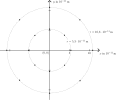
\includegraphics{images/diagram.pdf}
  \end{center}
\end{document}
